\section{Results}
\label{sec:results}

All members are scored on 8 to 10 July 2025, the intersection of their
post-spinup spans, which contains the whole drifter record.

\subsection{Water level}
\label{sec:res_wl}

Raw error at the three interior stations (Table~\ref{tab:wl}) is dominated by
a bias that all members share, positive at the North Mouth and AltaVilaEst,
between 0.03 and 0.09~m, and negative at the South Mouth, between $-0.051$ and
$-0.015$~m, which is a property of the datum and the boundary offset rather
than a difference between members.

Across the four members the anomaly RMSE varies by 1.6~mm at the South Mouth
(Figure~\ref{fig:wl}b), and by 12~mm at the North Mouth, where it follows wave
coupling,
falling from 0.039 to 0.027~m without a canopy and from 0.038 to 0.031~m with
one. At AltaVilaEst, the innermost station, in the northern basin where the
meadow is densest, it varies by 32~mm and follows the canopy, the vegetated
members giving 0.021 and 0.028~m with correlations of 0.94 and 0.95 and the
bare members 0.048 and 0.054~m with correlations of 0.79 and 0.81. There the
bare members overshoot the range of the observed anomaly and run ahead of it,
most visibly on the falling limb of 9 July, while the vegetated ones track both
amplitude and phase (Figure~\ref{fig:wl}a). With the canopy also in the wave
model, \texttt{WV}$^{\mathrm{s}}$ gives an anomaly RMSE of 0.026~m and a
correlation of 0.94 at AltaVilaEst, and 0.038~m at the North Mouth, the value
of the uncoupled members. A segment restarted without any change reproduces its
continuous member in water level and drifter skill (Section~S6), so the
separation at AltaVilaEst does not reflect the restart.

\begin{figure}[H]
  \centering
  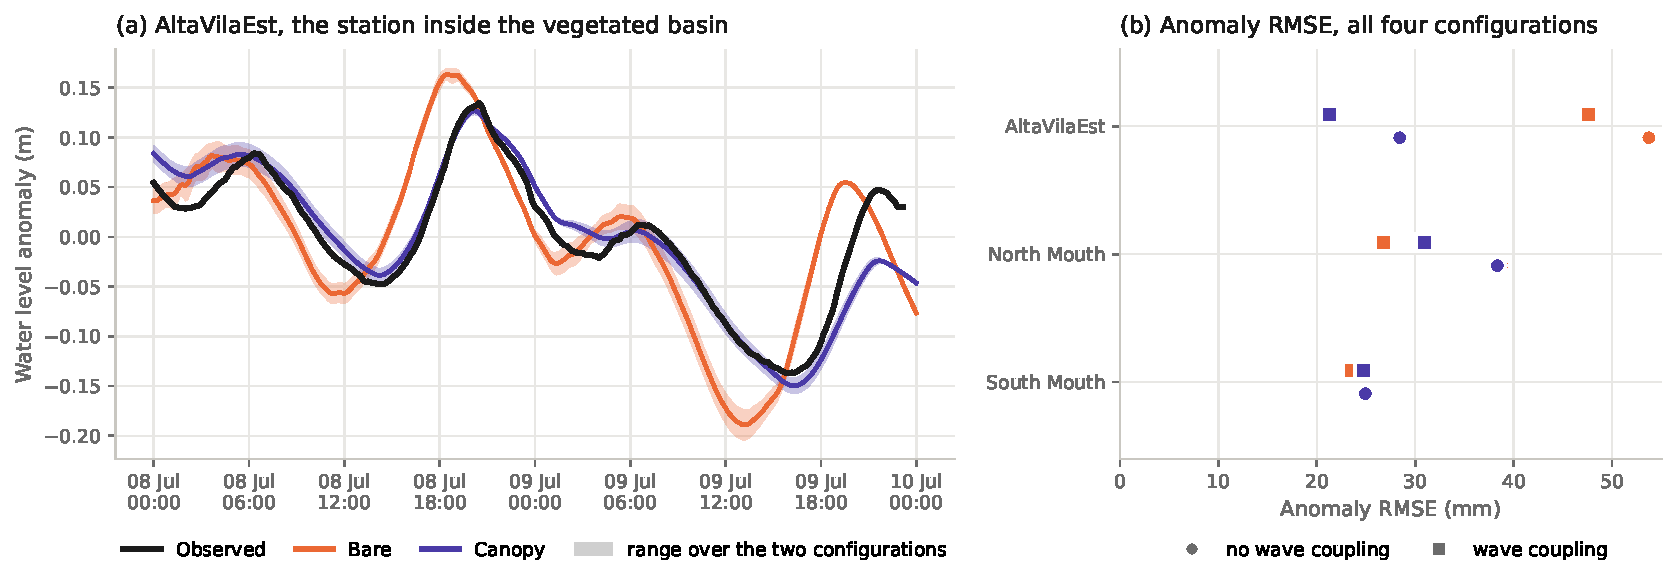
\includegraphics[width=\textwidth]{water_level_stations}
  \caption{Water level over the scored window. (a) Anomaly at AltaVilaEst,
  observed against the bare and the vegetated members, each pair drawn as its
  mean and range. Anomalies are shown rather than raw levels, the bias being
  common to all members. (b) Anomaly RMSE at the three stations for every
  member, coloured by canopy treatment, with circles for the uncoupled and
  squares for the wave-coupled members. The two uncoupled members nearly
  coincide at the North and South Mouths.}
  \label{fig:wl}
\end{figure}

\begin{table}[H]
  \centering
  \caption{Water level skill by member and station, 8--10 July 2025.
  $\mathrm{RMSE}^2 = \mathrm{bias}^2 + \mathrm{RMSE}_{\mathrm{anom}}^2$. Members
  are coded by wave coupling (W) and seagrass canopy (V). All values in metres
  except the dimensionless ratios.}
  \label{tab:wl}
  \begin{tabular}{llrrrrr}
    \toprule
    Station & Member & RMSE & Bias & RMSE$_{\mathrm{anom}}$ & $r$ & $\sigma_m/\sigma_o$ \\
    \midrule
    North Mouth & \texttt{{-}{-}} & 0.052 & $+0.035$ & 0.039 & 0.89 & 1.20 \\
                & \texttt{{-}V}   & 0.050 & $+0.033$ & 0.038 & 0.90 & 1.22 \\
                & \texttt{W{-}}   & 0.065 & $+0.059$ & 0.027 & 0.94 & 1.08 \\
                & \texttt{WV}     & 0.059 & $+0.051$ & 0.031 & 0.92 & 1.09 \\
    \midrule
    South Mouth & \texttt{{-}{-}} & 0.050 & $-0.043$ & 0.025 & 0.95 & 1.20 \\
                & \texttt{{-}V}   & 0.057 & $-0.051$ & 0.025 & 0.95 & 1.16 \\
                & \texttt{W{-}}   & 0.028 & $-0.015$ & 0.024 & 0.94 & 1.06 \\
                & \texttt{WV}     & 0.035 & $-0.025$ & 0.025 & 0.93 & 1.02 \\
    \midrule
    AltaVilaEst & \texttt{{-}{-}} & 0.076 & $+0.053$ & 0.054 & 0.81 & 1.37 \\
                & \texttt{{-}V}   & 0.049 & $+0.040$ & 0.028 & 0.94 & 1.18 \\
                & \texttt{W{-}}   & 0.097 & $+0.085$ & 0.048 & 0.79 & 1.18 \\
                & \texttt{WV}     & 0.070 & $+0.067$ & 0.021 & 0.95 & 1.01 \\
    \bottomrule
  \end{tabular}
\end{table}

\subsection{Lagrangian transport}
\label{sec:res_drifters}

Thirty-five drifters over twelve deployments were scored against each member
(Table~\ref{tab:lagrangian}, Figure~\ref{fig:lagrangian}). Mean Liu--Weisberg
skill spans 0.597 to 0.739 and endpoint separation 327 to 481~m, and the
members divide on the canopy without overlap, the vegetated ones scoring 0.711
and 0.739 and the bare ones 0.597 and 0.619. Both components of the trajectory
error improve with the canopy, the path length ratio rising from 0.80 and 0.83
to 0.88 and 0.94 and the mean heading error falling from 11.2 and
10.4$^\circ$ to 8.5 and 8.4$^\circ$. With the canopy also in the wave model,
the wave-coupled vegetated member scores 0.734.

\begin{table}[H]
  \centering
  \caption{Lagrangian metrics by member, 35 drifters over twelve deployments,
  scored on the interval each drifter was in the water. Path ratio is
  simulated over observed path length. Heading error is the mean angular
  difference between simulated and observed step directions, computed on
  eleven deployments since deployment 4 has too few positions to form the
  three step bearings it requires. \texttt{WV}$^{\mathrm{s}}$ carries the
  canopy in the wave model as well.}
  \label{tab:lagrangian}
  \begin{tabular}{lccrrrr}
    \toprule
    Member & Waves & Canopy & LW skill & Endpoint (m) & Path & Heading \\
    \midrule
    \texttt{{-}{-}} & no  & no  & 0.619 & 478 & 0.80 & 11.2$^\circ$ \\
    \texttt{{-}V}   & no  & yes & \textbf{0.739} & \textbf{327} & 0.88 & 8.5$^\circ$ \\
    \texttt{W{-}}   & yes & no  & 0.597 & 481 & 0.83 & 10.4$^\circ$ \\
    \texttt{WV}     & yes & yes & 0.711 & 335 & \textbf{0.94} & \textbf{8.4}$^\circ$ \\
    \texttt{WV}$^{\mathrm{s}}$ & yes & yes & 0.734 & 337 & 0.89 & \textbf{8.4}$^\circ$ \\
    \bottomrule
  \end{tabular}
\end{table}

\begin{figure}[H]
  \centering
  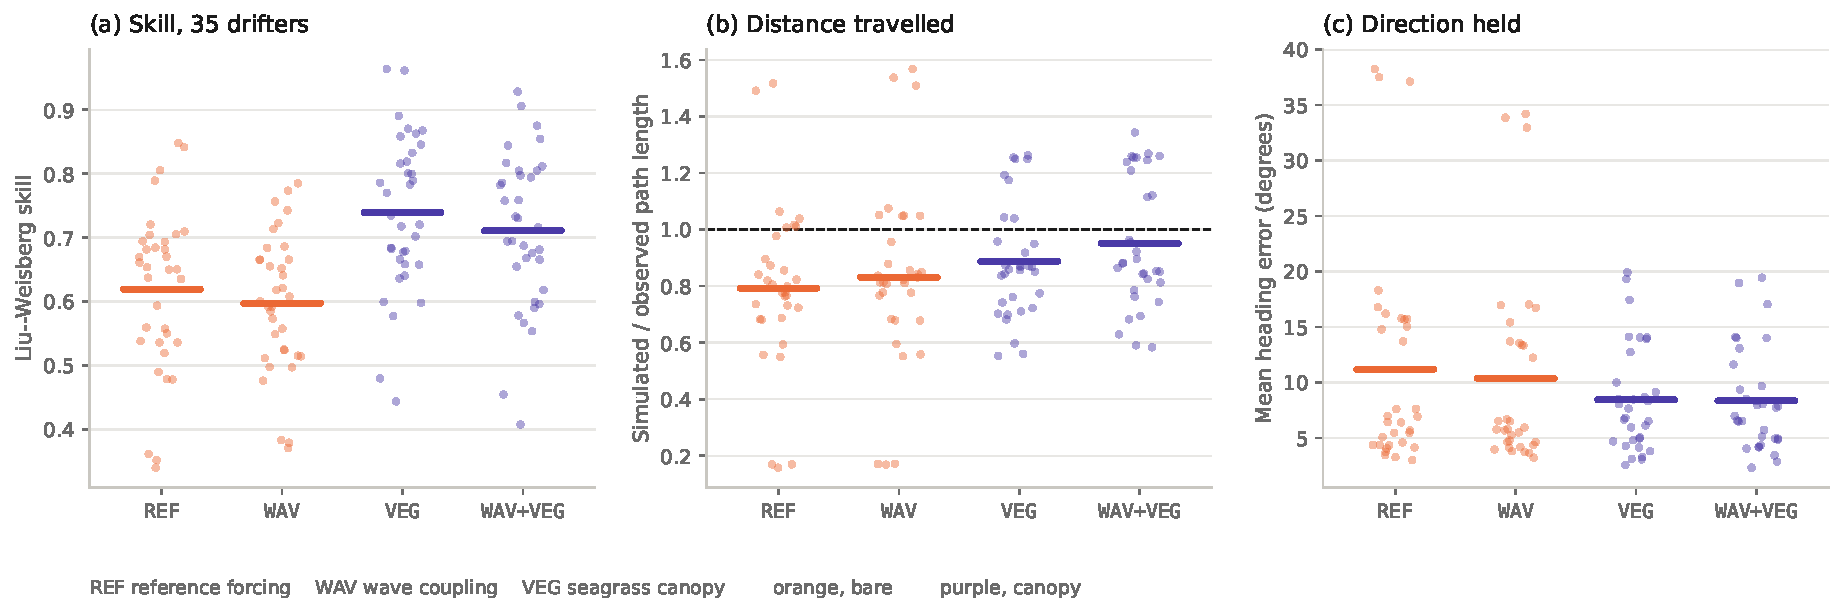
\includegraphics[width=\textwidth]{lagrangian_results}
  \caption{Lagrangian validation, one point per drifter and the bar giving the
  mean. (a) Liu--Weisberg skill. (b) Simulated over observed path length, the
  dashed line marking equality. (c) Mean angular difference between simulated
  and observed step directions. Panels (b) and (c) carry 32 drifters, since
  deployment 4 has too few positions to form step bearings.}
  \label{fig:lagrangian}
\end{figure}

In the tracks of the wave-coupled pair (Figure~\ref{fig:tracks}), the bare
particles of deployments 1 to 3 leave the observed path early and finish short
of the observed endpoint while the vegetated ones hold its heading. In the
deployments that drifted south, 8 to 12, both members follow the observed path
closely. Deployment 4, the shortest record at 0.4~h, is the one in which the
bare member ends nearer the observed endpoint.

\begin{figure}[H]
  \centering
  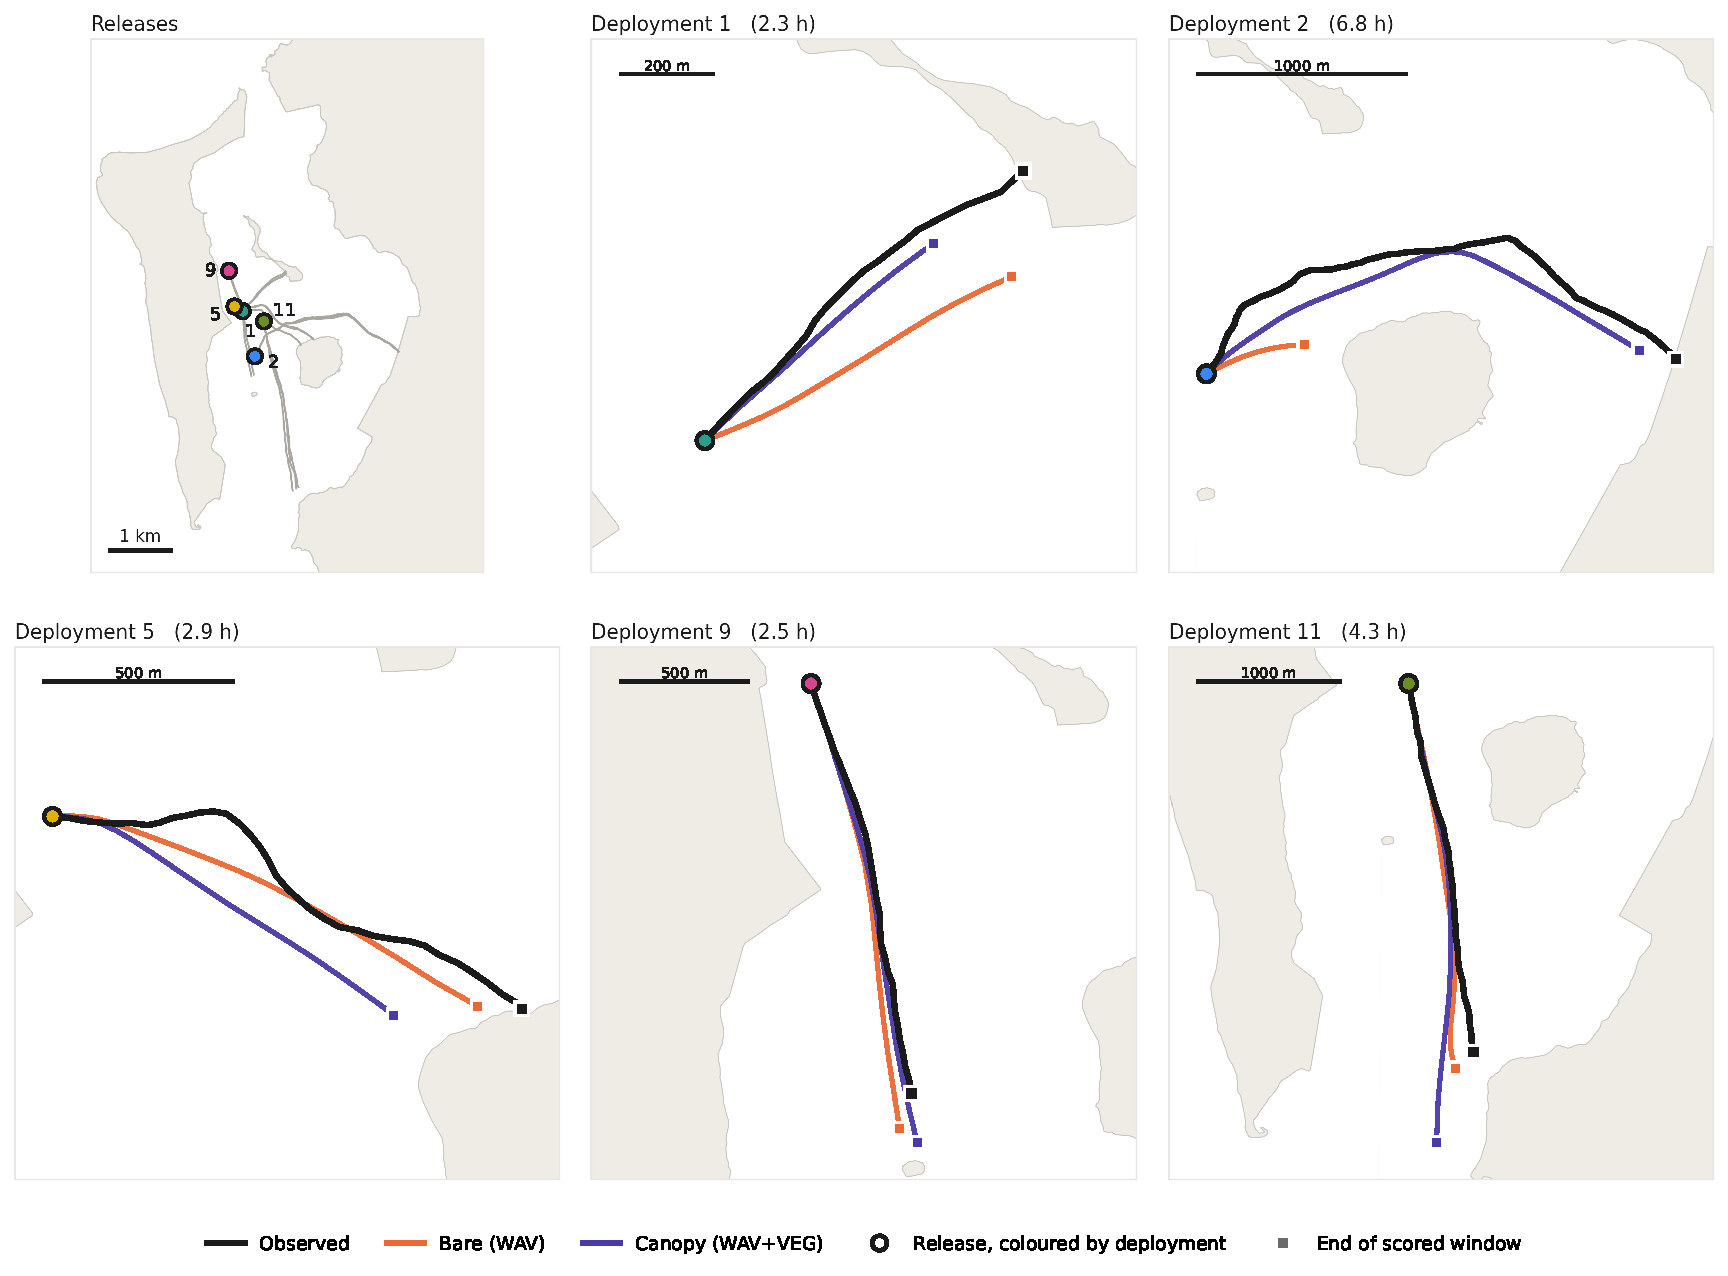
\includegraphics[width=\textwidth]{drifter_trajectories}
  \caption{Observed and simulated drifter trajectories for the two
  wave-coupled members that differ only in the canopy, \texttt{W{-}} and
  \texttt{WV}. The left panel numbers the release of each deployment over the
  observed tracks of all 35 drifters. Each deployment panel shows the
  median-skill drifter of that deployment under \texttt{WV}, with circles
  marking the release and squares the end of the scored window, each track
  clipped to the interval its drifter was in the water. Panel extents differ,
  so each carries its own scale bar.}
  \label{fig:tracks}
\end{figure}

\subsection{Process attribution}
\label{sec:res_attribution}

The two-factor design gives two single-factor contrasts per factor, each
measuring one factor with the other held at one of its levels
(Section~\ref{sec:methods_validation}). In the interaction plot of
Figure~\ref{fig:attribution}a the rise from bare bed to canopy is the canopy
effect and the gap between the two lines the wave effect, and
Figure~\ref{fig:attribution}b gives the contrasts with their bootstrap
intervals.

The canopy raises skill by 0.120 (95\% CI $+0.061$ to $+0.180$) without wave
coupling and by 0.114 ($+0.057$ to $+0.169$) with it, with 25 and 27 of the 35
drifters improving. The two contrasts agree to within 0.006, so the canopy
effect does not depend on the wave treatment, and the two lines of
Figure~\ref{fig:attribution}a run nearly parallel.

Wave coupling lowers skill by 0.022 ($-0.044$ to $-0.002$) without a canopy and
by 0.028 ($-0.040$ to $-0.017$) with one, with 21 and 25 drifters worse, an
effect about a fifth of that of the canopy. With the canopy also dissipating
wave energy, \texttt{WV}$^{\mathrm{s}}$ scores 0.023 above \texttt{WV}
($+0.014$ to $+0.031$), the wave contrast under the canopy falls to $-0.005$
($-0.011$ to $-0.001$) and the canopy contrast with waves rises to $+0.137$
($+0.084$ to $+0.194$), while significant wave height over the vegetated points
falls to a median of 0.36 of its bare-bed value (Section~S2). Most of the wave
penalty under the canopy therefore came from a wave field computed over a bare
bed.

The canopy contrast keeps the same sign under both wave treatments in ten of
the twelve deployments (Figure~\ref{fig:attribution}c). Deployment 4, the
shortest record and the one in which the bare members score higher, is
retained, and excluding it raises the two canopy contrasts to $+0.148$ and
$+0.144$ (Section~S6).

\begin{figure}[H]
  \centering
  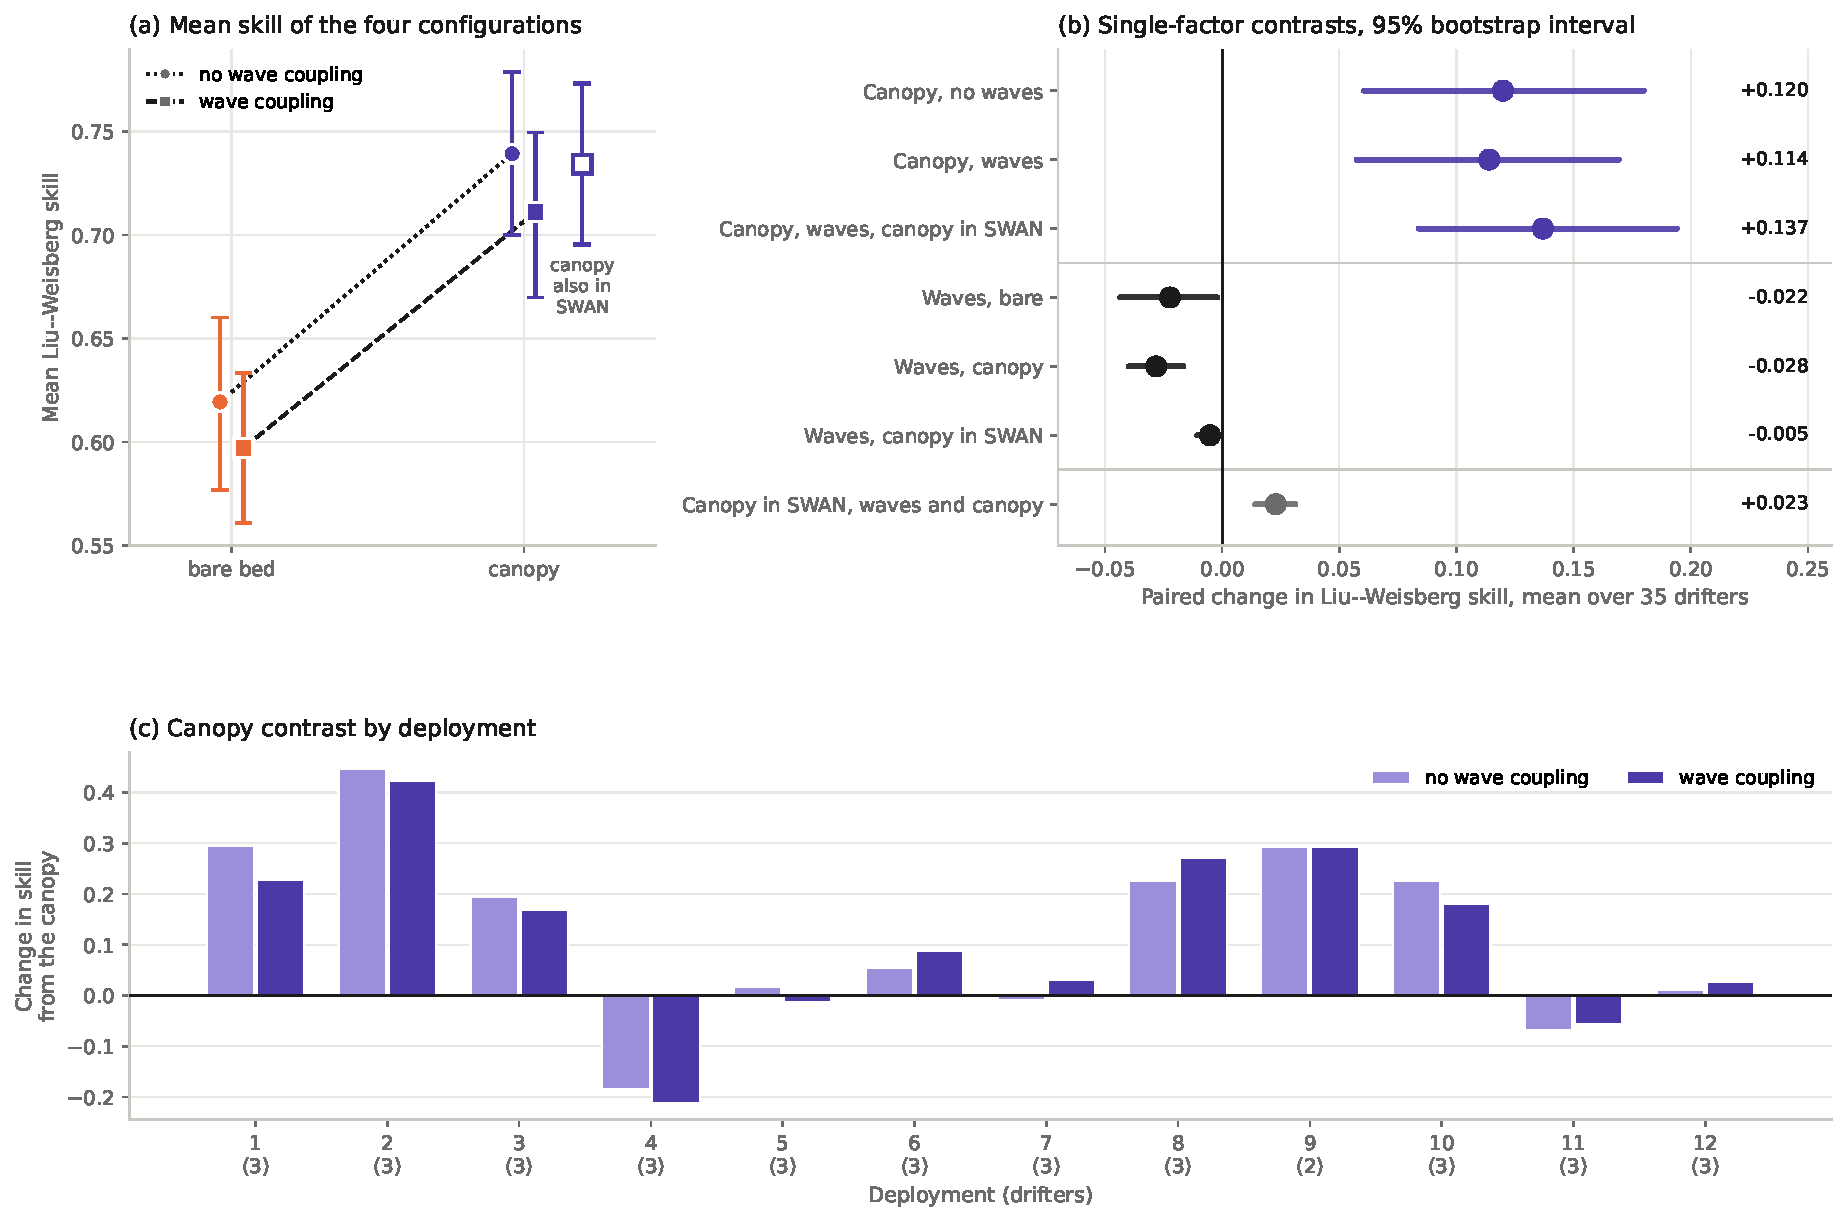
\includegraphics[width=\textwidth]{ensemble_attribution}
  \caption{Process attribution over the 35 drifters. (a) Mean Liu--Weisberg
  skill of the four members with 95\% bootstrap intervals, lines joining the
  members of equal wave treatment, and \texttt{WV}$^{\mathrm{s}}$ as the open
  square beside \texttt{WV}. (b) Single-factor contrasts, each the mean of the
  per-drifter paired differences in skill, with 95\% percentile bootstrap
  intervals from 4000 resamples, filled markers denoting intervals clear of
  zero. (c) The canopy contrast by deployment, without and with wave coupling,
  with the number of drifters per deployment in parentheses.}
  \label{fig:attribution}
\end{figure}

\subsection{Three-dimensional structure}
\label{sec:res_3d}

Over the wet cells of the lagoon interior, inlets excluded, mean current speed
increases monotonically from bed to surface in every member, and the canopy
sets the shape of that profile (Figure~\ref{fig:profile}). Without a canopy,
bed-layer speed is 0.032 to 0.035~\si{\metre\per\second} and surface-layer
speed 0.065 to 0.069~\si{\metre\per\second}, for surface-to-bed ratios of 1.88
and 2.14. With a canopy, bed-layer speed falls to 0.0093 to
0.0095~\si{\metre\per\second} while surface speed falls much less, to 0.043 to
0.047~\si{\metre\per\second}, and the ratio rises to 4.50 and 5.05. Wave
coupling adds 0.26 to the ratio without a canopy and 0.55 with one, against a
canopy contribution of $+2.62$ without waves and $+2.91$ with them.

Bed shear stress averaged over the meadow on 8 July fell from 0.028 to
0.0026~\si{\pascal} when the canopy was introduced, a factor of 11, whereas a
diagnostic run representing the same meadow as an equivalent bed roughness,
through the trachytope formulation of \citet{Baptist2007}, raised it to
0.043~\si{\pascal} over the same cells and times. Lagoon-mean surface speed
does not order the members as transport does, the best-scoring member having
the lowest surface speed, 0.043~\si{\metre\per\second}, against
0.069~\si{\metre\per\second} for a member whose particles travel 17\% too short
a distance.

\begin{figure}[H]
  \centering
  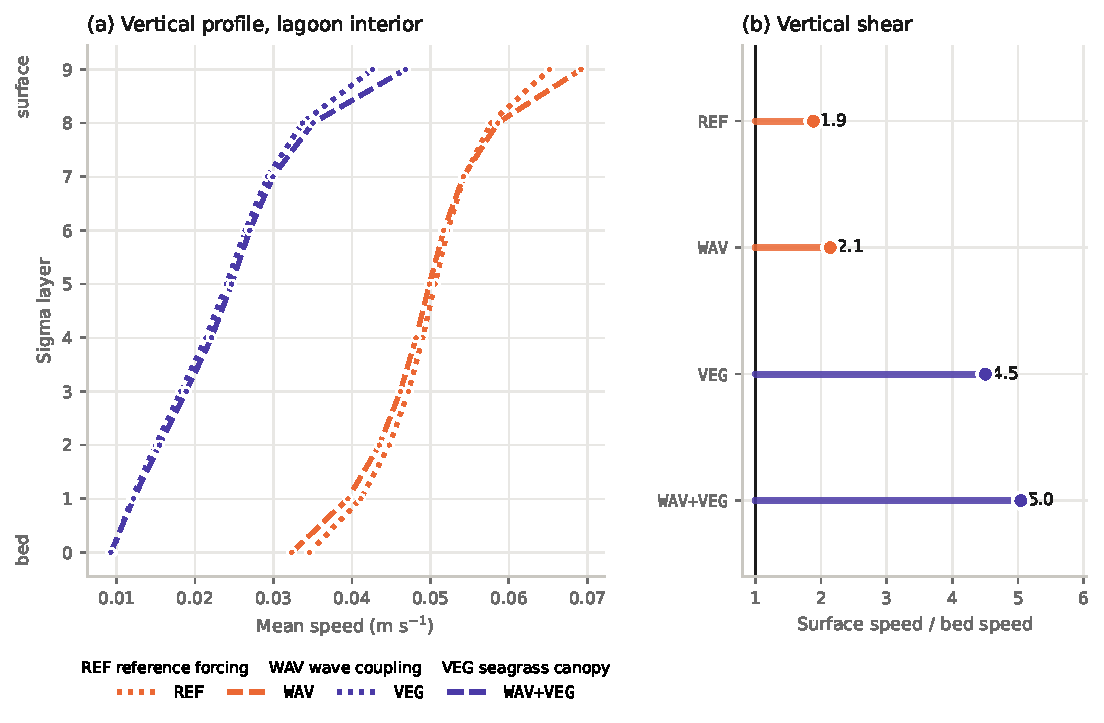
\includegraphics[width=0.88\textwidth]{layer_profile_lagoon}
  \caption{Vertical structure in the lagoon interior over the drifter window.
  (a) Mean speed by sigma layer, colour giving the canopy treatment and line
  style the wave treatment. (b) Ratio of surface to bed speed.}
  \label{fig:profile}
\end{figure}

\subsection{Sensitivity to the initial condition and the discretisation}
\label{sec:res_sensitivity}

Started from a vertically uniform column instead of the stratified state, the
bare members score 0.080 and 0.092 lower and the vegetated members 0.005 and
0.018 lower, so that the canopy contrasts become $+0.195$ and $+0.188$. The
uniform start raises the modelled mean water level at the gauges by 2 to 10~cm
and changes anomaly RMSE by at most 4~mm and correlation by at most 0.03, and
the canopy signature at AltaVilaEst is the same under both starts.

The horizontal and vertical resolution, the time-step limit and the host and
decomposition change skill by less than 0.01 under a Courant limit of 0.5 and
water level by at most 2.4~mm (Section~S5). Under the Courant limit of 0.7 used
by the ensemble, the uncoupled bare member scores $0.034 \pm 0.004$ lower on
four partitions on a second computer than on eight on the server, a dependence
that all members share.
